\documentclass[t,9pt]{beamer}

\usetheme{CambridgeUS}
\usecolortheme{seahorse}

\setbeamertemplate{navigation symbols}{}
\setbeamertemplate{section in toc}[ball unnumbered]

\usefonttheme{serif}
\usepackage{newtxmath}
\usepackage[onehalfspacing]{setspace}

\usepackage[ngerman]{babel}
\usepackage{amsmath,amssymb,amsfonts}
\usepackage{siunitx}
\usepackage[absolute,overlay]{textpos}
\usepackage{bookmark}
\usepackage{csquotes}

\usepackage[framemethod=TikZ]{mdframed}
\usepackage{tcolorbox}
\tcbuselibrary{theorems}
\tcbuselibrary{skins}

\newcommand{\td}{\text{d}}

\newcommand{\highlight}[3]{ \begin{textblock*}{#1}(#2,#3) \begin{tcolorbox} [enhanced,opacityfill=.1,colback=blue] \end{tcolorbox} \end{textblock*} } % \highlight{100pt}{10pt}{25pt}

\title[\thesection]{Das magnetische Moment des Protons}
\subtitle{Proseminar Präsentationstechnik c \\\tiny Prof.\ Dr.\ Harmut Schmieden}
\author{Jonas Wortmann}
\institute{Universität Bonn}
\date{\today}
\logo{\LaTeX{}}

\begin{document}

        \AddToHook{shipout/foreground}{
          \begin{tikzpicture}[remember picture,overlay]
            \node[red,rotate=30,scale=5,opacity=0.1] at (current page.center) {Draft};
          \end{tikzpicture}
        }

        \begin{frame}
                \titlepage
        \end{frame}

        \begin{frame}{Inhaltsverzeichnis}
                \tableofcontents[pausesections]
        \end{frame}

        \section{Entdeckung des Protons}

        \begin{frame}{Inhaltsverzeichnis}
                \tableofcontents[currentsection]
        \end{frame}

        \begin{frame}{Entdeckung des Protons}
                % TODO WIEN CHARGE MASS RATIO; GOLDSTEIN H+; RUTHERFORD UNTER ANDEREM BEKANNT FÜR BENENNUNG
                1913 \textsc{Mardsen}: Wasserstoff wird mit $\alpha $--Teilchen beschossen.
                \begin{itemize}
                        \item Aufblitzen auf einem Zinksulfidschirm in \textbf{großer Distanz} (zu kurz für $\alpha $).
                        \item Aufblitzen von \textbf{H--Atomen} verursacht.
                \end{itemize}
                \pause
                \vspace{.5cm} \textsc{Rutherford}: Stickstoff wird mit $\alpha $--Teilchen beschossen.
                \begin{itemize}
                        \item Aufblitzen von \textbf{H--Atomen} verursacht.
                                \pause
                        \item Stickstoff muss \textbf{H--Atome als Bestandteile} besitzen.
                \end{itemize}
                \pause
                \vspace{.5cm}1920 \textsc{Rutherford}: \textbf{Jedes} Atom muss aus \textbf{H--Atomen} (Protonen) bestehen.\cite{Rutherford_proton_discovery}
        \end{frame}


        \begin{frame}{Endteckung des Protons}
                \begin{figure}
                        \highlight{100pt}{255pt}{2.3cm}
                        \highlight{190pt}{8pt}{2.8cm}
                        \highlight{120pt}{45pt}{3.2cm}
                        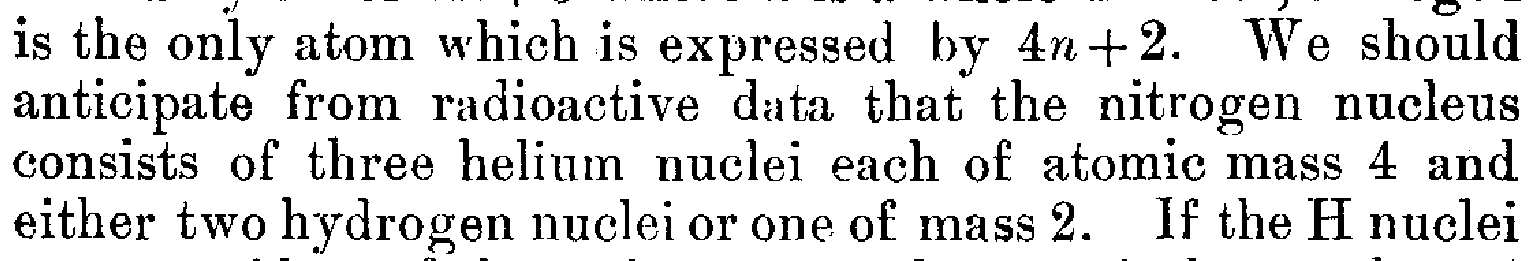
\includegraphics[width=\textwidth]{prosi_nitrogen_made_of_H.png}
                        \caption{Auszug: Stickstoff besteht aus Wasserstoff.\cite{Rutherford1919}}
                \end{figure}
        \end{frame}

        \begin{frame}{Endteckung des Protons}
                \begin{figure}
                        \highlight{205pt}{155pt}{3.2cm}
                        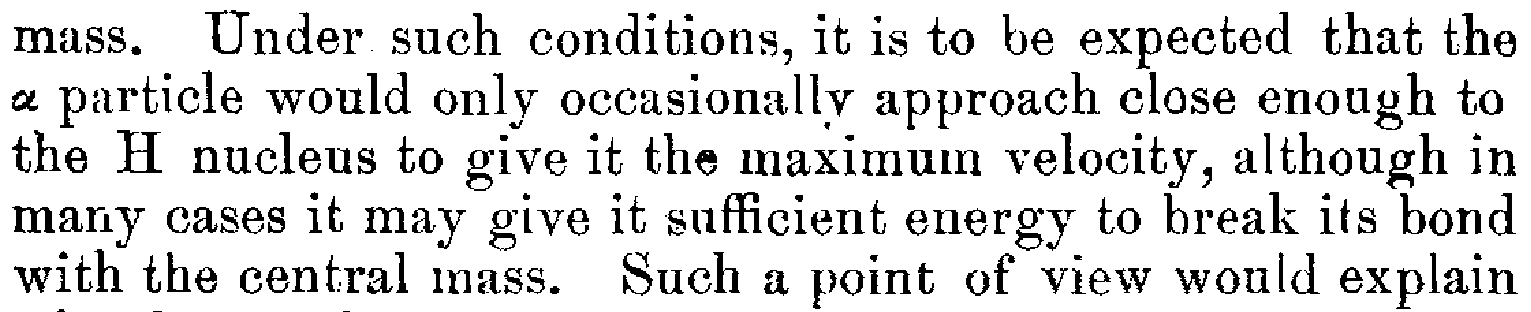
\includegraphics[width=\textwidth]{prosi_alpha_breaks_H_from_nitrogen.png}
                        \caption{Auszug: $\alpha $--Teilchen hebt Bindung von Stickstoff auf.\cite{Rutherford1919}}
                \end{figure}
        \end{frame}

        \begin{frame}{Endteckung des Protons}
                \begin{figure}
                        \highlight{250pt}{60pt}{2.8cm}
                        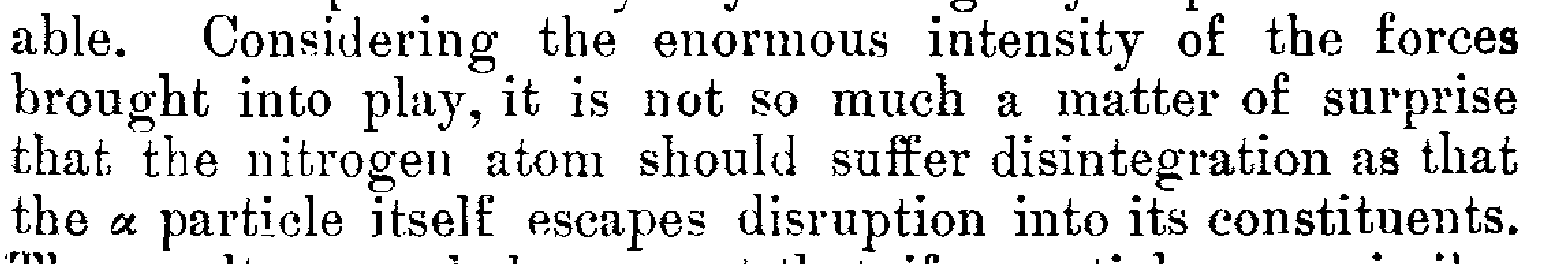
\includegraphics[width=\textwidth]{prosi_nitrogen_disintegrates.png}
                        \caption{Auszug: Stickstoff desintegriert.\cite{Rutherford1919}}
                \end{figure}
        \end{frame}

        \section{Magnetisches (Dipol--)Moment}

        \begin{frame}{Inhaltsverzeichnis}
                \tableofcontents[currentsection]
        \end{frame}

        \begin{frame}{Magnetisches (Dipol--)Moment}
                Magnetisches Moment gibt \textbf{Stärke} und \textbf{Richtung} eines magnetischen Dipols an.
                \begin{center}
                        \tcboxmath[colframe=white]{\boldsymbol{m}=\dfrac{1}{2}\int_{}^{}\td ^3r\left[\boldsymbol{r}\times \boldsymbol{j}\left(\boldsymbol{r}\right)\right]\qquad \vv{m}=I\cdot\boldsymbol{A}}
                \end{center}
                \pause
                Klassische / Quantenmechanische Betrachtung mit \textbf{Drehimpuls}:
                \begin{center}
                        \tcboxmath[colframe=white]{\boldsymbol{\mu}_l=\dfrac{q}{2m_q}\boldsymbol{l} \qquad \boldsymbol{\hat{\mu}}_q=\dfrac{q}{2m_q}\hat{\boldsymbol{l}} \qquad {\boldsymbol{\hat{\mu}}}_s=g_s\dfrac{q}{2m_q}{\boldsymbol{\hat{s}}}}
                \end{center}
                \pause
                \textsc{Bohr}'sche Magneton (Elektronen $\ell=1$) \& Kernmagneton (\textsc{Dirac}--Teilchen)
                \begin{center}
                        \tcboxmath[colframe=white]{\mu _B=\dfrac{e\hbar }{2m_e}\qquad \mu _N=\dfrac{e\hbar }{2m_p}}
                \end{center}
        \end{frame}

        \section{Das Proton als Elementarteilchen}

        \begin{frame}{Inhaltsverzeichnis}
                \tableofcontents[currentsection]
        \end{frame}

        \begin{frame}{Das Proton als Elementarteilchen}
                \textsc{Dirac}--Theorie: 
                \begin{center}
                        \tcboxmath[colframe=white]{\left(\text{i}\gamma ^\mu \partial_\mu -m\right)\phi \left(\boldsymbol{x} ,t\right)=0}
                \end{center}
                Lösungen sind erlaubte Zustände elementarer Fermionen.
                \pause
                \\\vspace{.5cm} Proton als \textsc{Dirac}--Teilchen:
                \begin{center}
                        \tcboxmath[colframe=white]{\mu _p=1\mu _N=1\dfrac{e\hbar }{2m_p}\approx \SI{5.505e-27}{J/T}}
                \end{center}
                \tiny\vspace{-.2cm}\hspace{8.1cm}CODATA\cite{CODATA_nuclear_magneton}\normalsize
        \end{frame}

        \begin{frame}{Das Proton als Elementarteilchen}
                \begin{figure}
                        \highlight{118pt}{240pt}{4.2cm}
                        \highlight{205pt}{5pt}{4.7cm}
                        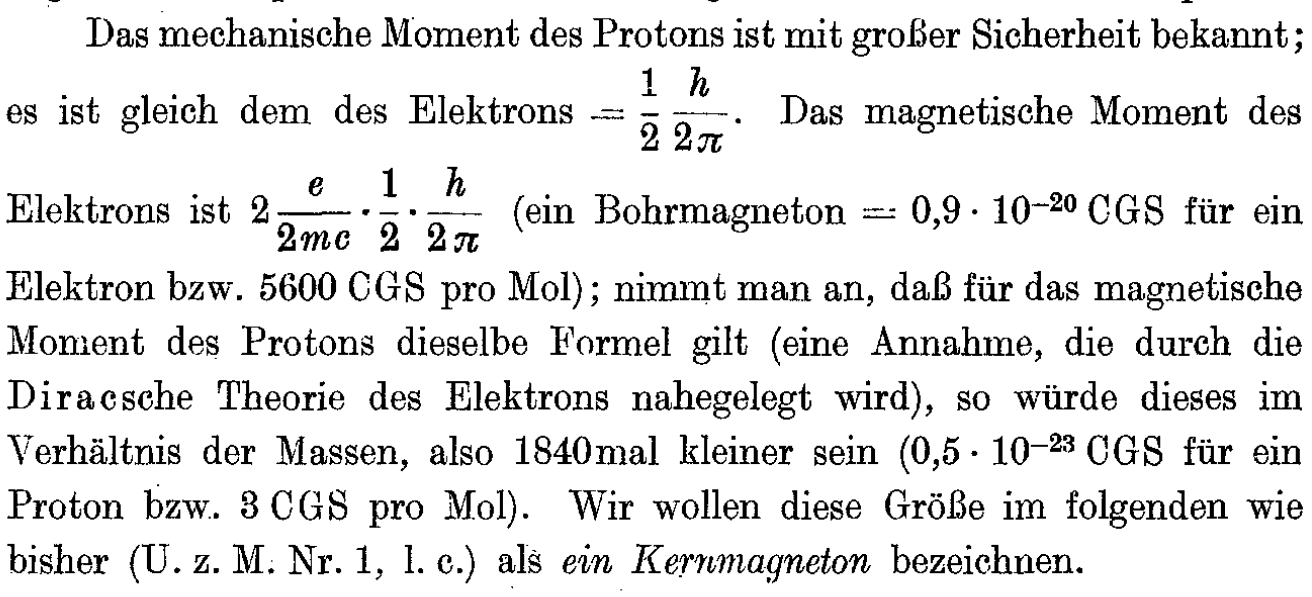
\includegraphics[width=\textwidth]{prosi_proton_als_dirac_teilchen.png}
                        \caption{Auszug: Proton als \textsc{Dirac}--Teilchen.\cite{FrischStern1933}}
                \end{figure}
        \end{frame}

        \section{Experiment Otto Robert \textsc{Frisch} \& Otto \textsc{Stern}} 

        \begin{frame}{Inhaltsverzeichnis}
                \tableofcontents[currentsection]
        \end{frame}

        \begin{frame}{Experiment Otto Robert \textsc{Frisch} \& Otto \textsc{Stern}}
                \begin{figure}
                        \highlight{6.4cm}{6.1cm}{2.3cm}
                        \highlight{1.8cm}{.3cm}{2.8cm}
                        \highlight{7.4cm}{5.2cm}{4.3cm}
                        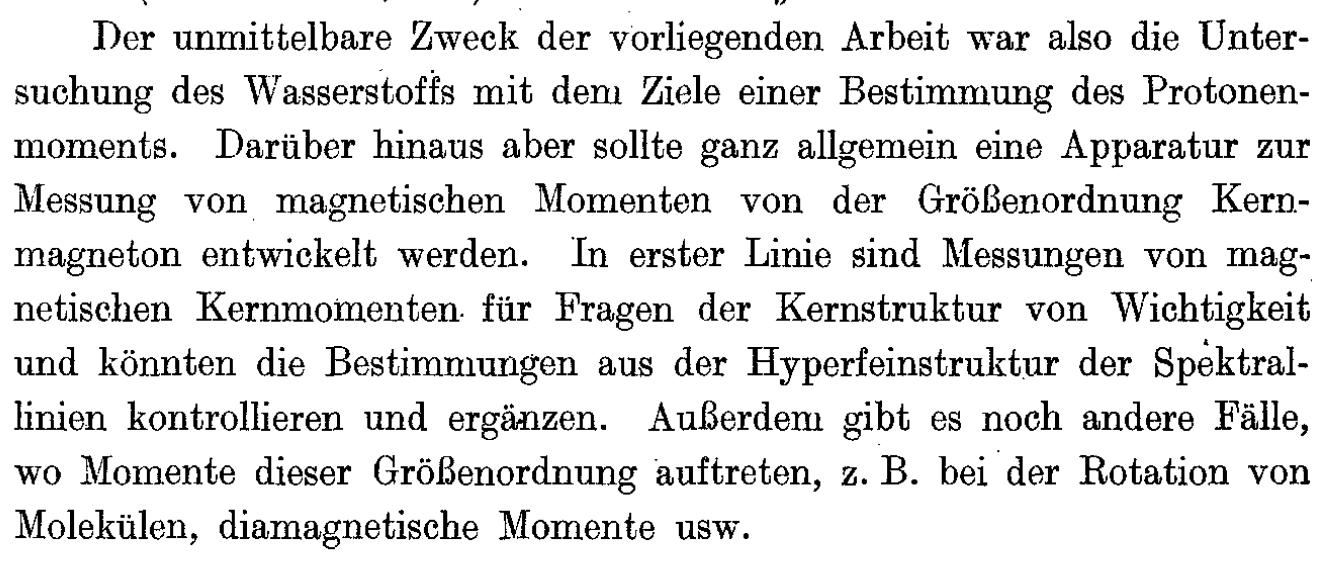
\includegraphics[width=\textwidth]{prosi_zweck_der_arbeit.png}        
                        \caption{Auszug: Ziel des Experiments.\cite{FrischStern1933}}
                \end{figure}
        \end{frame}

        \begin{frame}{Experiment Otto Robert \textsc{Frisch} \& Otto \textsc{Stern}}
                \begin{figure}
                        \highlight{4.1cm}{1.5cm}{2.9cm}
                        \highlight{12.3cm}{.2cm}{3.4cm}
                        \includegraphics[width=\textwidth]{prosi_mag_moment_großes_interesse.png}
                        \caption{Auszug: Magnetisches Moment von Interesse.\cite{FrischStern1933}}
                \end{figure}
        \end{frame}

        \begin{frame}{Experiment Otto Robert \textsc{Frisch} \& Otto \textsc{Stern}} 
                \begin{figure}
                        \highlight{3.8cm}{8.7cm}{1.75cm}
                        \highlight{2.1cm}{.2cm}{2.1cm}
                        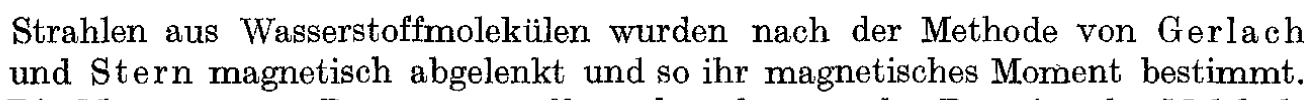
\includegraphics[width=\textwidth]{prosi_nach_methode_stern_gerlach.png}
                        \caption{Auszug: Methoden nach \textsc{Gerlach} und \textsc{Stern}.\cite{FrischStern1933}}
                \end{figure} 
                \begin{figure}
                        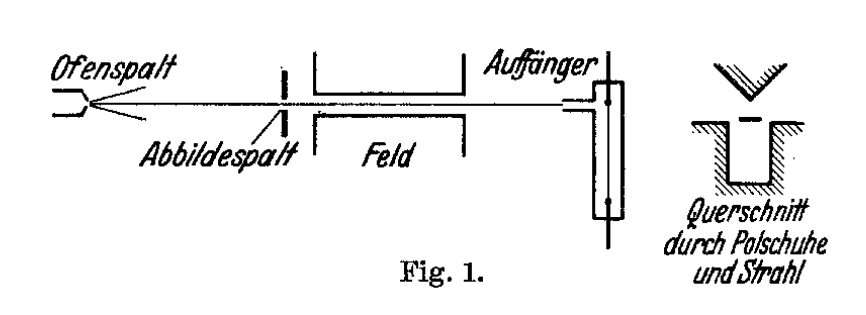
\includegraphics[width=.8\textwidth]{prosi_versuchsaufbau_mag_moment.png}
                        \caption{Versuchsaufbau zur Messung des magnetischen Moments. Gesamtlänge des Aufbaus ca.\ $\SI{30}{cm}$.\cite{FrischStern1933}}
                \end{figure}
        \end{frame}

        \begin{frame}{Experiment Otto Robert \textsc{Frisch} \& Otto \textsc{Stern}\cite{FrischStern1933}}
                Anforderungen zur Messung kleiner magnetischer Momente:\\
                \begin{itemize}
                        \item Strahl muss \textbf{lang} und \textbf{schmal} sein (kleinster Strahl ca.\ $\SI{0.03}{mm}$).
                        \item \textbf{Große Inhomogenität} des Feldes (ca.\ $\SI{2.2e+5}{Gs/cm}=\SI{22}{T/cm}$).
                \end{itemize}
                \pause
                \vspace{.5cm} Die Ablenkung des Strahls für 1 Kernmagneton liegt bei $s\approx \SI{0.044}{mm}$.
                \pause
                \\\vspace{.5cm}Schwierigkeiten:
                \begin{itemize}
                        \item Der Strahl ist \textbf{nicht monochromatisch}, sondern \textsc{Maxwell}--verteilt. Das gesuchte magnetische Moment muss aus der \textbf{Intensitätsverteilung} erschlossen werden.
                        \item Wegen der großen Länge und geringen Höhe war die \textbf{Intensität klein}.
                \end{itemize}
        \end{frame}

        \begin{frame}{Experiment Otto Robert \textsc{Frisch} \& Otto \textsc{Stern}\cite{FrischStern1933}}
                Ergebnisse:
                \begin{itemize}
                        \item Parahelium hat kein magnetisches Moment.
                                \pause
                        \item Aufhebung der Entartung der Drehimpulsquantenzahl von Orthohelium.
                \end{itemize}
                \pause
                \begin{figure}
                        \highlight{4.8cm}{.9cm}{4.5cm}
                        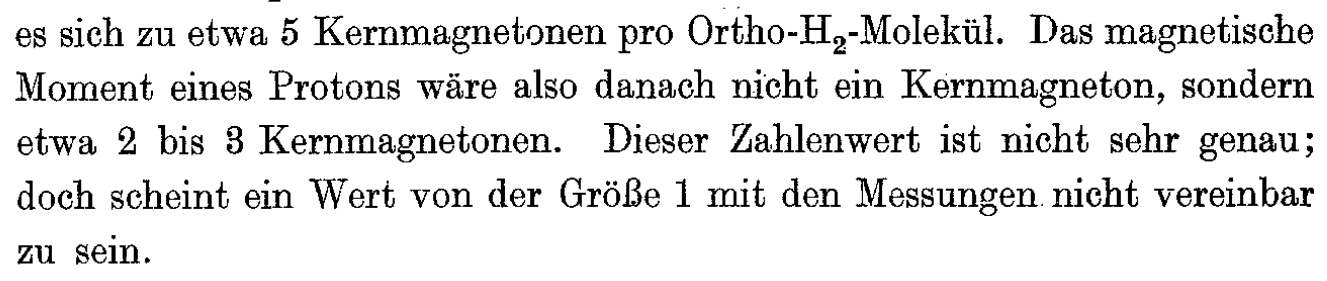
\includegraphics[width=.9\textwidth]{prosi_mag_moment_proton_nicht_1.png}
                        \caption{Auszug: Das Ergebnis des magnetischen Moments.\cite{FrischStern1933}}
                \end{figure}
        \end{frame}

        \section{Die Substruktur des Protons}

        \begin{frame}{Inhaltsverzeichnis}
                \tableofcontents[currentsection]
        \end{frame}

        \begin{frame}{Die Substruktur des Protons}
                Einteilung der Teilchen in Hadronen: %TODO (BILD MIT 3 HALBKUGELN BOSON HADRON FERMION)        
                \\\vspace{.1cm} $\rightarrow $ Baryon: Fermion aus 3 Quarks
                \\ $\rightarrow $ Meson: Boson aus 2 Quarks
                %TODO BILD PAPER GELL MANN ZWEIG
        \end{frame}

        \section{SLAC Experiment}

        \begin{frame}{Inhaltsverzeichnis}
                \tableofcontents[currentsection]
        \end{frame}

        \begin{frame}{SLAC Experiment}
                \pause
                Elektronen streuen an Nukleonen mit \textbf{großen Winkeln}. % TODO BILD HISTORY STANDARD MODEL / SLAC
                \\\vspace{.1cm} $\rightarrow $ Analogie \textsc{Rutherford}: Nukleonen haben eine punktförmige \textbf{Substruktur}.
                \pause
                \\\vspace{.5cm} Interpretation \textsc{Feynman} \& \textsc{Bjorken}: Proton besteht aus \textbf{Partonen}.
                \\\vspace{.1cm} $\rightarrow $ Partonen sind als \textsc{Gell-Mann}s \& \textsc{Zweig}s \textbf{Quarks} zu identifizieren. %TODO BILD PAPER
        \end{frame} 

        \section{Das Proton als Baryon}

        \begin{frame}{Inhaltsverzeichnis}
                \tableofcontents[currentsection]
        \end{frame}

        \begin{frame}{Das Proton als Baryon}
                \pause
                Das Proton ist \textit{kein} elementares Fermion, sondern ein \textbf{Baryon} (u,u,d).
                \pause
                \begin{center}
                        \tcboxmath[colframe=white]{\mu _p=\dfrac{3}{4}\mu _u-\dfrac{1}{3}\mu _d \approx 2.792\,\mu _N\approx \SI{1.410e-27}{J/T}}
                \end{center}
                \tiny\vspace{-.2cm}\hspace{8.8cm}CODATA\cite{CODATA_proton_magneton}\normalsize
                \pause
                \\ Differenz: 
                \begin{center}
                        \tcboxmath[colframe=white]{|\,\mu _\text{PF}-\mu _\text{PB}\,|\approx \SI{4.095e-27}{J/T}}
                \end{center}
        \end{frame}

        \section{Ausblick}

        \begin{frame}{Inhaltsverzeichnis}
                \tableofcontents[currentsection]
        \end{frame}

        \begin{frame}{Ausblick}
                \pause
                Magnetresonanztomographie        
        \end{frame}

        \begin{frame}{Bibliography}
                \tiny
                \bibliographystyle{plain}
                \bibliography{refs}
        \end{frame}
                
\end{document}
